\documentclass[10pt,journal]{IEEEtran}

\usepackage[T1]{fontenc}
\usepackage[utf8]{inputenc}
\usepackage{microtype}
\usepackage{amsmath,amssymb,amsthm,mathtools,bm}
\usepackage{booktabs,tabularx,array,multirow}
\usepackage{algorithm}
\usepackage[noend]{algpseudocode}
\usepackage{graphicx}
\usepackage{dblfloatfix}
\usepackage{xcolor}
\usepackage{cite}
\usepackage{xurl}
\usepackage[hidelinks]{hyperref}
\usepackage{tikz}
\usetikzlibrary{arrows.meta,positioning,fit,calc,shapes.geometric,patterns}

\interdisplaylinepenalty=2500
\allowdisplaybreaks
\emergencystretch=2em
\setlength{\textfloatsep}{5pt plus 1pt minus 1pt}
\setlength{\floatsep}{5pt plus 1pt minus 1pt}
\setlength{\dblfloatsep}{4pt plus 1pt minus 1pt}
\setlength{\dbltextfloatsep}{5pt plus 1pt minus 1pt}
\setlength{\intextsep}{5pt plus 1pt minus 1pt}
\setlength{\abovecaptionskip}{3pt}
\setlength{\belowcaptionskip}{0pt}

\newtheorem{proposition}{Proposition}
\newtheorem{theorem}{Theorem}
\newtheorem{corollary}{Corollary}
\newtheorem{remark}{Remark}

\DeclareMathOperator*{\argmin}{arg\,min}
\newcommand{\R}{\mathbb{R}}
\newcommand{\one}{\mathbf{1}}
\newcommand{\pos}[1]{\left[#1\right]_+}
\newcommand{\Mone}{\ensuremath{\mathrm{M1}}}
\newcommand{\MoneLP}{\ensuremath{\mathrm{M1\text{-}LP}}}
\newcommand{\Mtwo}{\ensuremath{\mathrm{M2}}}
\newcommand{\Mthree}{\ensuremath{\mathrm{M3}}}
\newcommand{\MtwoMatched}{\ensuremath{\mathrm{M2\text{-}MATCHED}}}
\newcommand{\lexleq}{\preceq_{\mathrm{lex}}}
\newcommand{\FDE}{\ensuremath{\mathrm{FDE}}}

% The final campaign writes results_final.tex and sets \FinalResultsReadytrue.
% Fallback definitions keep the paper compilable before that file exists.
\newif\ifFinalResultsReady
\FinalResultsReadyfalse
\IfFileExists{results_final.tex}{\input{results_final.tex}}{}
\providecommand{\HeldMTwoS}{--}
\providecommand{\HeldMTwoRhoThreeS}{--}
\providecommand{\HeldMOneLower}{--}
\providecommand{\HeldMOneUpper}{--}
\providecommand{\HeldCertMargin}{--}
\providecommand{\ConfirmMTwoS}{--}
\providecommand{\ConfirmMOneLower}{--}
\providecommand{\ConfirmMOneUpper}{--}
\providecommand{\HeldMTwoE}{--}
\providecommand{\HeldMThreeS}{--}
\providecommand{\HeldMMatchedS}{--}
\providecommand{\HeldMThreeFDE}{--}
\providecommand{\HeldMMatchedFDE}{--}
\providecommand{\HeldMThreeBurden}{--}
\providecommand{\HeldMMatchedBurden}{--}
\providecommand{\HeldRollingMOneS}{--}
\providecommand{\HeldRollingMTwoS}{--}
\providecommand{\HeldRollingMThreeS}{--}
\providecommand{\IndependentDCMaxError}{--}
\providecommand{\IndependentDCFalseSafe}{--}
\providecommand{\SelectedACConvergence}{--}
\providecommand{\SelectedACReversals}{--}
\providecommand{\AnnualRuntimeRange}{--}
\providecommand{\RollingRuntimeRange}{--}

\title{Annual Entitlement Accounting for Partial Restrictions in Non-Firm Transmission Access: A Dutch Transmission Study}

\author{Alban Kryeziu, Stuart X.~Zhu, Tolga Karabas, and Evrim Ursavas%
\thanks{The authors are with the Department of Operations, Faculty of Economics and Business, University of Groningen, 9747 AE Groningen, The Netherlands. Corresponding author: Alban Kryeziu (e-mail: a.kryeziu@rug.nl).}}

\begin{document}
\maketitle

\begin{abstract}
A non-firm transmission contract can permit partial restriction while limiting how much intervention may be used over a year. The unresolved design question is the debit unit: should a partially restricted interval consume one unit of touched time, or only the restricted fraction of contracted capacity? These rules protect different services and create different intertemporal feasible sets. We formulate a common contingency-aware restriction-allocation problem and compare touched-time accounting (M1), proportional-depth accounting (M2), and a frozen state-conditioned depth rule (M3). The continuous M1 relaxation admits an exact projection. Its feasible set is contained in the M2 set under the same physical model and allowance, which yields a strict Stage-I certificate against every feasible annual M1 schedule without requiring a global solution of the annual M1 mixed-integer problem. M3 is constructed from one exact Stage-II M2 primal--dual pair in each fitting year, uses only predeclared D--1-admissible features, and is frozen before held-out evaluation. An ex-post M2-MATCHED problem separates changed physical exposure from state allocation. The study uses 61,344 hourly intervals, a 45-bus Dutch EHV model, 79 directly represented positions, 95 monitored elements, and the intact state plus 93 retained non-islanding outages. Province-level demand, PV, onshore wind, and offshore wind are projected separately to buses before the security-adjusted background state is formed. Numerical statements are admitted only after independent replay, an independent selected-state DC reconstruction, and selected-state nonlinear stress checks.
\ifFinalResultsReady
Across the held-out years, M2 attains a Stage-I value of \HeldMTwoS\ MW\,h\,row-state while the annual M1 optimum is certified in [\HeldMOneLower,\,\HeldMOneUpper], with a strict margin of \HeldCertMargin.
\fi
\end{abstract}

\begin{IEEEkeywords}
Annual entitlement, congestion management, flexible connections, non-firm transmission access, rolling-horizon optimization, transmission security.
\end{IEEEkeywords}

\section{Introduction}
\label{sec:introduction}

A system operator that grants non-firm transmission access must answer two different questions. The first is physical: which restriction relieves the network state? The second is contractual: how much of a participant's finite annual entitlement does that restriction consume? The second question becomes material as soon as restriction is divisible. If a 100-MW position is reduced by 5 MW in one interval and by 100 MW in another, a touched-time rule charges both intervals once after a materiality threshold is crossed. A proportional rule charges $0.05$ and $1.00$ full-depth-equivalent intervals. Once the first interval is opened under touched time, additional depth is free in entitlement units even though its network effect continues to change. The debit law therefore links today's physical action to the set of actions available in later congestion states.

Non-firm and flexible connection agreements are used to provide access before reinforcement is available, and prior work studies offered capacity, curtailment risk, priority rules, activation, and network-aware flexibility allocation \cite{AnayaPollitt2015,DzamarijaKeane2013,HubertColey2021,Bjarghov2024,DeSanti2025,Monterde2025,SeifertBjarghovBakker2026}. Related models coordinate connection limitations with redispatch or markets \cite{Oikonomou2020,Tsaousoglou2021,VanDerHolst2024Activation,VanDerHolst2026RiskAware}. Contract-design studies examine interruptible service, intervention rights, duration, participation, and incentives \cite{ChaoWilson1987,ChaoWilson1990,OrenSmith1992,CavesHerriges1992,FahriogluAlvarado2000,Nouicer2023}. These streams determine which action may be taken or how the right to interrupt should be allocated. They generally take the resource-consumption map of an implemented partial restriction as given.

This paper holds the requests, eligibility set, physical evaluator, ratings, allowance vector, and operator objective fixed and changes only that map. The Dutch time-duration transport right provides the immediate setting: it protects transport availability over a declared annual fraction while partial restriction remains operationally meaningful \cite{ACM2024ATR,ACM2026TDTR}. The analysis does not reproduce the full legal, settlement, or dispute framework. It isolates the operational consequence of defining one unit of annual entitlement as touched duration rather than normalized physical depth.

Touched-time accounting (M1) limits materially affected participant--interval coordinates. It protects intervention frequency but is depth-blind after a coordinate is opened. It also requires binary support decisions and makes the annual model large. Proportional-depth accounting (M2) charges $x/P$, where $x$ is restricted MW and $P$ is contracted MW. The debit is divisible and additive in physical exposure. We derive the exact projection of the continuous M1 relaxation and prove
\begin{equation}
\Pi\mathcal F_y^{\Mone}(\bm H)
\subseteq
\mathcal F_y^{\MoneLP}(\bm H)
\subseteq
\mathcal F_y^{\Mtwo}(\bm H).
\label{eq:intro_hierarchy}
\end{equation}
The mechanism is a denominator change. The M1 relaxation divides each restriction by the currently available request bound $\bar x_{n,t}$; M2 divides it by the contracted capacity $P_n\geq \bar x_{n,t}$. Hence M2 never charges more depth than the projected M1 relaxation at the same action.

The inclusion resolves the main computational obstruction. A time-limited M1 incumbent cannot establish that M2 outperforms every feasible annual M1 schedule. In contrast, M1-LP supplies a certified lower bound on the annual M1 Stage-I optimum, and a complete rolling-M1 trajectory supplies an implementable upper endpoint. If a replay-feasible M2 value lies strictly below the M1-LP lower bound after numerical margins, then M2 is strictly better in Stage I than every feasible annual M1 schedule. This is an annual scalar certificate. Hourly cumulative curves may explain chronology, but they are not pointwise bounds on an unknown annual M1 optimum.

We also examine whether the depth debit should vary with the operating state. M3 multiplies $x/P$ by a bounded rate fixed before operation. The rate card is learned offline from selected Stage-II M2 scarcity attributions; it does not predict or choose the restriction. Candidate cards are fitted on 2025--2027, compared on 2028, and frozen before 2029--2031 are opened. Because a nonuniform card may change the unweighted physical exposure available under the same nominal allowance, M3 is always compared with M2-MATCHED, which grants each participant the physical full-depth-equivalent exposure realized by M3 and then re-solves uniform-depth accounting. This separates an entitlement-exposure effect from the residual state-shape effect.

The Dutch study is not a single national load trace attached to a network. Demand, PV, onshore wind, and offshore wind remain separate at province or landing-point level and are projected through technology-specific matrices to the retained EHV buses. Bounded generation and signed net-boundary injections then produce a security-adjusted background state. A 383-bus mixed-voltage model supports localization and reduction checks; a 45-bus 220/380-kV model supports the chronological policy problems. The predeclared all-or-none mapping gate rejects the 35 multibus embeddings from the primary case, leaving 79 positions represented directly at retained EHV buses. The physical evaluator covers 95 monitored elements in the intact state and 93 retained non-islanding single-element outages, yielding 8,837 state--element rows per hour.

The paper makes four contributions. First, it formulates annual restriction entitlement as an operational state and separates the services protected by touched duration and normalized physical exposure. Second, it derives the exact M1-LP projection, the feasible-set hierarchy in \eqref{eq:intro_hierarchy}, and a strict certificate that compares M2 or a fixed-card M3 policy with every annual M1 schedule without claiming a solved annual M1 mixed-integer optimum. Third, it defines an allowance-specific, nonanticipative M3 construction based on one exact Stage-II M2 primal--dual pair, a provenance gate, a fit--validate--freeze split, and matched-exposure diagnosis. PTDF, inverse, and frozen shuffle controls test whether any effect is specific to the selected ordering. Fourth, it builds an auditable Dutch physical case from separate component trajectories, technology-specific bus projections, bounded background balancing, retained outage states, and a fail-closed detailed-to-reduced participant gate. Independent row replay, an independent DC software path, and selected-state AC checks place explicit limits on the physical claims.

The central contribution is the M1--M2 accounting geometry and certificate. M3 is a secondary mechanism test. The remainder of the paper defines the common operator problem, proves the accounting results, specifies the frozen card, documents the Dutch construction, and sets out the evidence required for the numerical conclusions.

\section{Common Operator Problem and Debit Rules}
\label{sec:model}

\subsection{Requests, restrictions, and balanced network states}

Let $y\in\mathcal Y$ index years, $t\in\mathcal T_y$ hourly intervals, $n\in\mathcal N$ directional non-firm positions, $b\in\mathcal B$ buses, and $c\in\mathcal C$ retained network states. Every interval retains an explicit duration $\Delta_t>0$, although the final case uses $\Delta_t=1$ h. Position $n$ has contracted capacity $P_n>0$, requested transport $y^{\rm req}_{n,t}\geq0$, contract-duration indicator $\kappa_{n,t}\in\{0,1\}$, and restriction-eligibility indicator $\chi_{n,t}\in\{0,1\}$. The model requires $\chi_{n,t}\leq\kappa_{n,t}$ but does not infer contract duration, eligibility, and positive request from one another. In particular, zero request does not shorten the contract duration used to compute the annual allowance.

The operator chooses the withheld quantity $x_{n,t}$,
\begin{equation}
0\leq x_{n,t}\leq \bar x_{n,t}:=
\chi_{n,t}\min\{P_n,y^{\rm req}_{n,t}\}.
\label{eq:xbar}
\end{equation}
Let $\bm p_t^{\rm bg}\in\R^{B}$ be the balanced background injection before prospective non-firm requests. Let $\bm A=[\bm a_1,\ldots,\bm a_N]$ be the participant transaction matrix. The vector $-\bm a_n$ is the nodal change caused by one MW of requested transport; $+\bm a_n$ reverses one MW when the request is restricted. The same counter-injection convention is used for every accounting rule, with
\begin{equation}
\one^\top\bm p_t^{\rm bg}=0,
\qquad
\one^\top\bm A=\bm0^\top.
\label{eq:balance}
\end{equation}
The requested and post-restriction states are
\begin{align}
\bm p_t^{\rm req}
&=\bm p_t^{\rm bg}-\bm A\bm y_t^{\rm req},
\notag\\
\bm p_t(\bm x)
&=\bm p_t^{\rm req}+\bm A\bm x_t.
\label{eq:nodal_state}
\end{align}
The parent model contains restriction only. Redispatch is not allowed to differ across debit rules and is considered, when data support it, only as a common post-policy engineering test. The model has no storage state of charge, generator ramping, or unit-commitment logic. The only intertemporal state in the policy problem is the annual entitlement balance. The background builder uses hour-specific bounded device ranges but does not claim chronological unit commitment.

For state $c$, the retained affine DC evaluator is
\begin{equation}
\bm f_t^c=\bm H^c\bm p_t(\bm x)+\bm h^c,
\label{eq:affine_dc}
\end{equation}
where $\bm h^c$ preserves fixed phase-shift and other affine terms. For monitored element $r\in\mathcal R_c$ with declared rating $\bar F_r^c>0$,
\begin{equation}
-\bar F_r^c-s^-_{r,t,c}
\leq f^c_{r,t}\leq
\bar F_r^c+s^+_{r,t,c},
\qquad s^\pm_{r,t,c}\geq0.
\label{eq:security}
\end{equation}
The claim is limited to the intact state and the retained, mapped, non-islanding single-element outages of the reduced EHV model. Equation \eqref{eq:security} is not an AC-OPF model and is not presented as full Dutch N--1 certification.

\subsection{Lexicographic objective}

Every debit rule enters the same sequential operator problem. Stage I minimizes integrated directed thermal-row slack,
\begin{equation}
S(\bm x,\bm s)
:=\sum_{t\in\mathcal T_y}\Delta_t
\sum_{c\in\mathcal C}\sum_{r\in\mathcal R_c}
\left(s^+_{r,t,c}+s^-_{r,t,c}\right).
\label{eq:stage1}
\end{equation}
The unit is MW$\cdot$h$\cdot$row-state. The quantity is a residual-violation index for the declared evaluator; it is not curtailed energy, redispatch cost, welfare, customer compensation, or a monetary benefit. Let $S_y^{M,\star}$ be the certified Stage-I value under rule $M$. Stage II minimizes restricted energy on the Stage-I-optimal face,
\begin{align}
E_y^{M,\star}:=
\min_{(\bm x,\bm s)\in\mathcal X_y\cap\mathcal D_y^M}
&\ \sum_{n,t}\Delta_t x_{n,t}
\notag\\
\mathrm{s.t.}\quad
&S(\bm x,\bm s)
\leq S_y^{M,\star}+\varepsilon_S.
\label{eq:stage2}
\end{align}
The reported value is
\begin{equation}
\mathcal V_y^M=(S_y^{M,\star},E_y^{M,\star}),
\label{eq:value}
\end{equation}
ordered lexicographically. The sequence avoids an arbitrary conversion between MW$\cdot$h$\cdot$row-state and MWh: avoidable row violations are removed before intervention volume is compared. When a canonical policy vector is needed for a figure or engineering state selection, an optional third solve may fix both values and apply a deterministic selector. That selector is not part of \eqref{eq:value}, is not required for the M1--M2 certificate, and is not used for the M3 teacher. The primary annual and rolling production runs therefore require only certified Stages I and II unless a downstream artifact explicitly needs a selected point on the optimal face.

\subsection{Allowance and accounting services}

On the hourly grid, participant $n$ receives
\begin{align}
N_{n,y}^{\rm ctr}&:=\sum_t\kappa_{n,t},
&K_{n,y}(\rho)&:=\left\lfloor\rho N_{n,y}^{\rm ctr}\right\rfloor,
\notag\\[-1mm]
H_{n,y}&:=K_{n,y}(\rho)\Delta.
&&
\label{eq:allowance}
\end{align}
Same-scale comparisons use the same serialized vector $\bm H_y$ and vector hash. The floor is part of the contract definition; it is not replaced by a ceiling or by $\rho$ times the number of positive requests.

M1 introduces $u_{n,t}\in\{0,1\}$ and a materiality floor
\begin{equation}
\underline x_{n,t}:=
\min\{\bar x_{n,t},\max(1\ {\rm MW},0.01P_n)\}.
\label{eq:floor}
\end{equation}
Its constraints are
\begin{equation}
\underline x_{n,t}u_{n,t}\leq x_{n,t}
\leq\bar x_{n,t}u_{n,t},
\qquad
\sum_t\Delta_tu_{n,t}\leq H_{n,y}.
\label{eq:m1}
\end{equation}
The threshold defines the counted contractual action, not numerical zero.

M2 and M3 use
\begin{align}
D_{n,y}^{2}(\bm x)
&:=\sum_t\Delta_t\frac{x_{n,t}}{P_n}\leq H_{n,y},
\notag\\
D_{n,y}^{3}(\bm x;\bm q)
&:=\sum_t\Delta_tq_{n,t}\frac{x_{n,t}}{P_n}\leq H_{n,y},
\qquad q_{n,t}>0.
\label{eq:m2m3}
\end{align}
M2 protects cumulative normalized physical exposure. M3 changes the debit exchange rate applied to that exposure. It does not change the physical action bounds or choose $x$ outside the common operator problem.

\begin{table}[t]
\caption{Accounting services under a common physical model}
\label{tab:rules}
\centering
\footnotesize
\begin{tabularx}{\columnwidth}{@{}lXXX@{}}
\toprule
Rule & Debit & Protected service & Class \\
\midrule
M1 & $u_{n,t}$ & materially touched duration & MILP \\
M1-LP & $x_{n,t}/\bar x_{n,t}$ & projected touched-time relaxation & LP \\
M2 & $x_{n,t}/P_n$ & physical full-depth-equivalent exposure & LP \\
M3 & $q_{n,t}x_{n,t}/P_n$ & state-weighted physical exposure & LP after freeze \\
\bottomrule
\end{tabularx}
\end{table}

For fixed $P$, proportional depth is the only normalized additive physical-exposure debit under mild assumptions.

\begin{proposition}[Normalized additive depth]
\label{prop:m2_unique}
Let $d(\cdot;P):[0,P]\to\R_+$ satisfy $d(0;P)=0$, $d(P;P)=1$, monotonicity, and $d(x_1+x_2;P)=d(x_1;P)+d(x_2;P)$ whenever $x_1,x_2,x_1+x_2\in[0,P]$. Then $d(x;P)=x/P$.
\end{proposition}

The proof is given in the technical report. The proposition characterizes the unit; it does not assert that touched duration and physical depth are legally or economically equivalent.

\subsection{Rolling entitlement transition}

At rolling epoch $\tau$, let $\mathcal L_\tau$ be the 48-h look-ahead and $\mathcal I_\tau\subset\mathcal L_\tau$ the first 24 h that are implemented. Only the implemented block is charged:
\begin{align}
B_{n,\tau+1}^{M}
&=B_{n,\tau}^{M}
-\sum_{t\in\mathcal I_\tau}\Delta_t d_{n,t}^{M},
\label{eq:rolling}\\[-1mm]
d_{n,t}^{M}
&=
\begin{cases}
u_{n,t},&M=\Mone,\\
x_{n,t}/P_n,&M=\Mtwo,\\
q_{n,t}x_{n,t}/P_n,&M=\Mthree.
\end{cases}
\notag
\end{align}
The initial balance is $H_{n,y}$ in same-scale cases. The controller has no terminal reserve or terminal value. It is an unpaced receding-horizon policy, not an approximation guarantee for the annual optimum. Consecutive windows share 24 h; the implementation reuses the overlapping solution and previously discovered physical rows as computational starts, while every accepted epoch is reoptimized and replayed under its own balance.

\section{Entitlement Geometry and Certification}
\label{sec:geometry}

The distinction between M1 and M2 appears before the network enters. In the continuous M1 relaxation, a restriction $x_{n,t}$ requires at least the fraction $x_{n,t}/\bar x_{n,t}$ of an activation token. M2 charges the same action by $x_{n,t}/P_n$. Since $\bar x_{n,t}\leq P_n$, the projected M1 debit is never smaller.

\begin{theorem}[M1 projection, hierarchy, and strict certificate]
\label{thm:hierarchy}
Fix a year, a common physical set, and allowance vector $\bm H$. The projection of the continuous relaxation of \eqref{eq:m1} is
\begin{equation}
D_n^{1L}(\bm x):=
\sum_{t:\bar x_{n,t}>0}\Delta_t
\frac{x_{n,t}}{\bar x_{n,t}}
\leq H_n,
\qquad 0\leq x_{n,t}\leq\bar x_{n,t}.
\label{eq:m1lp}
\end{equation}
On a uniform grid with $H_n=K_n\Delta$ and integer $K_n$, \eqref{eq:m1lp} is the convex hull of the isolated participant-level M1 entitlement set. No convex-hull equality is asserted after intersection with the coupled network constraints. Moreover,
\begin{equation}
D_n^{1L}(\bm x)-D_n^2(\bm x)
=\sum_{t:\bar x_{n,t}>0}\Delta_t x_{n,t}
\left(\frac{1}{\bar x_{n,t}}-\frac{1}{P_n}\right)
\geq0.
\label{eq:debit_gap}
\end{equation}
Consequently,
\begin{align}
\Pi\mathcal F_y^{\Mone}(\bm H)
&\subseteq
\mathcal F_y^{\MoneLP}(\bm H)
\subseteq
\mathcal F_y^{\Mtwo}(\bm H),
\notag\\[-1mm]
\mathcal V_y^{\Mtwo}
&\lexleq
\mathcal V_y^{\MoneLP}
\lexleq
\mathcal V_y^{\Mone}.
\label{eq:set_value_hierarchy}
\end{align}
Let $Q$ be M2 or a fixed-card M3 problem with the same physical model and allowance. If $\overline S_y^Q$ is a replay-feasible Stage-I value, $\underline S_y^{1L}$ is a certified M1-LP lower bound, and
\begin{equation}
\overline S_y^Q+\varepsilon_{\rm cert}
<\underline S_y^{1L},
\label{eq:strict_certificate}
\end{equation}
then $S_y^{Q,\star}<S_y^{\Mone,\star}$.
\end{theorem}

\begin{IEEEproof}
For $\bar x_{n,t}>0$, the relaxed upper link in \eqref{eq:m1} gives $u_{n,t}\geq x_{n,t}/\bar x_{n,t}$. Setting equality also satisfies the lower link because $\underline x_{n,t}\leq\bar x_{n,t}$, which proves \eqref{eq:m1lp}. On a uniform grid, $z_t=x_{n,t}/\bar x_{n,t}$ lies in $\{0\leq z\leq1:\sum_tz_t\leq K_n\}$, the uniform-matroid independence polytope, whose extreme points are binary. Mapping a binary extreme point back by $x_{n,t}=\bar x_{n,t}z_t$ gives an isolated M1-feasible point. The qualification about network intersection follows because convexification does not generally commute with intersection.

Subtracting the M2 debit from \eqref{eq:m1lp} yields \eqref{eq:debit_gap}; every term is nonnegative. Relaxing integrality gives the first inclusion in \eqref{eq:set_value_hierarchy}, and the debit inequality gives the second. Lexicographic minimization over nested feasible sets yields the value ordering. Finally, $S_y^{Q,\star}\leq\overline S_y^Q$ and $\underline S_y^{1L}\leq S_y^{\MoneLP,\star}\leq S_y^{\Mone,\star}$, so \eqref{eq:strict_certificate} proves the strict result.
\end{IEEEproof}

\begin{figure}[t]
\centering
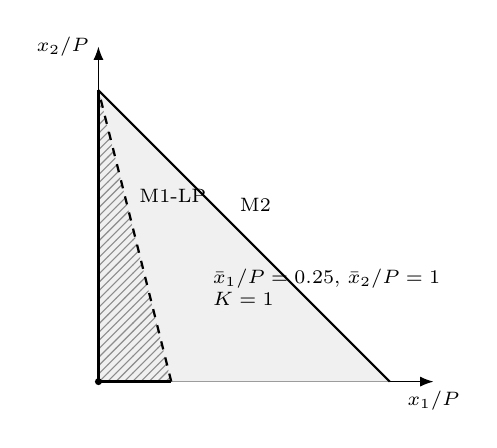
\begin{tikzpicture}[x=3.7cm,y=3.7cm,>=Latex,font=\scriptsize]
  \draw[->] (0,0) -- (1.15,0) node[below] {$x_1/P$};
  \draw[->] (0,0) -- (0,1.15) node[left] {$x_2/P$};
  \fill[black!6] (0,0)--(1,0)--(0,1)--cycle;
  \draw[thick] (1,0)--(0,1) node[pos=.55,above right] {M2};
  \fill[pattern=north east lines,pattern color=black!45]
    (0,0)--(.25,0)--(0,1)--cycle;
  \draw[thick,dashed] (.25,0)--(0,1)
    node[pos=.58,above right] {M1-LP};
  \draw[line width=1.2pt] (0,0)--(.25,0);
  \draw[line width=1.2pt] (0,0)--(0,1);
  \fill (0,0) circle (.012);
  \node[align=left,anchor=north west] at (.36,.42)
    {$\bar x_1/P=0.25$, $\bar x_2/P=1$\\$K=1$};
\end{tikzpicture}
\caption{Two-interval geometry for one participant. The projected M1 relaxation divides by the available request bound and forms the smaller triangle; M2 divides by contracted capacity. The isolated M1 projection is the union of the axis segments, whose convex hull is M1-LP. Coupled network constraints may cut all sets but do not reverse the inclusion.}
\label{fig:geometry}
\end{figure}

A completed rolling-M1 trajectory provides an annual feasible upper endpoint only when the implemented blocks form the full chronology without gaps or overlap, every block passes physical and debit replay, and the closing balances are nonnegative. Under these conditions,
\begin{equation}
S_y^{\Mtwo,\star}
\leq S_y^{\MoneLP,\star}
\leq S_y^{\Mone,\star}
\leq S_y^{\Mone,\mathrm{roll}}.
\label{eq:annual_bracket}
\end{equation}
The interval $[S_y^{\MoneLP,\star},S_y^{\Mone,\mathrm{roll}}]$ is an annual bracket. It does not imply that cumulative M1-LP violation is below cumulative rolling-M1 violation at every hour.

M2 is preserved by exact temporal aggregation. If a coarse interval of duration $\Delta$ contains subintervals $j$ of duration $\delta_j$ and $\bar x=\Delta^{-1}\sum_j\delta_jx_j$, then
\begin{equation}
\Delta\frac{\bar x}{P}
=\sum_j\delta_j\frac{x_j}{P}.
\label{eq:m2_aggregation}
\end{equation}
M1 is not average-preserving: four quarter-hour actions $(P,0,0,0)$ consume $0.25$ h of touched time on the fine grid, whereas their hourly average $P/4$ consumes one touched hour. M3 is additive on its native $(q,x)$ grid; a coarse rate preserves debit only when it is weighted by exposure.

\subsection{Exact constraint generation and replay}

The number of state--element--hour rows is too large to treat model assembly as a clerical detail. The implementation separates three sets. First, the complete action box determines which rows can ever be violated and which participant--hour actions can be removed by an exact dominance argument. Second, the initial optimization seed contains request-state violated and deterministically near-binding directed rows. Third, every omitted registered row remains in the closure and replay universe.

For $\bm G^c=\bm H^c\bm A$ and requested-state flow $f_{r,t}^{c,\rm req}$, the restriction box implies
\begin{align}
L_{r,t}^{c}
&=f_{r,t}^{c,\rm req}
+\sum_n\min\{0,G_{r,n}^c\bar x_{n,t}\},
\notag\\
U_{r,t}^{c}
&=f_{r,t}^{c,\rm req}
+\sum_n\max\{0,G_{r,n}^c\bar x_{n,t}\}.
\label{eq:screen_bounds}
\end{align}
A row--hour pair satisfying $L_{r,t}^{c}\geq-\bar F_r^c$ and $U_{r,t}^{c}\leq\bar F_r^c$ cannot be violated anywhere in the box and may be removed. Potentially active rows need not all enter the first model. Stage I is first closed at its own optimizer: the candidate is evaluated against every registered row and every omitted positive overload is added before the Stage-I value is accepted. Stage II is then solved on the certified Stage-I face. Its selected policy is again evaluated on the full physical evaluator. If the independently reconstructed $S$ lies outside the Stage-I face by more than the numerical comparison envelope, the implementation does not widen the lexicographic tolerance and does not project the solution after optimization. It first re-solves the identical model with stronger numerical arithmetic. If the violation persists, it adds a globally valid supporting inequality of the convex polyhedral function $S(\bm x)$ at the offending policy and re-solves Stage II. For a subgradient $\bm g^k\in\partial S(\bm x^k)$, the added inequality is
\begin{equation}
S(\bm x^k)+(\bm g^k)^\top(\bm x-\bm x^k)\leq S^{\rm cap}.
\label{eq:physical_face_cut}
\end{equation}
Every policy satisfying the true physical face $S(\bm x)\leq S^{\rm cap}$ satisfies \eqref{eq:physical_face_cut} by convexity, while the offending point is removed. Because $S$ is polyhedral, this is an exact outer-approximation mechanism rather than a heuristic repair. If a numerical recovery solve is required, only solver arithmetic is strengthened; the physical model, allowance, objectives, and scientific lexicographic tolerances are unchanged. The same replay guard applies to an optional Stage-III selector. The full proof and numerical contract are in the technical report.

Independent replay receives only immutable case objects and solution arrays. It reconstructs $\bar x$, M1 materiality, participant debits, rolling balance transitions, nodal injections, all affine flows, $S$, $E$, physical FDE, and the relevant hashes. Solver optimality alone is never used as the final feasibility certificate, and no accepted policy is modified after extraction from the optimization model.

\section{Frozen State-Conditioned Depth Accounting}
\label{sec:m3}

\subsection{Canonical teacher and information boundary}

M3 is allowance-specific and constructed offline. For fitting year $y$, the canonical M2 teacher solves Stage I and then the exact Stage-II LP on the replay-guarded Stage-I face. Let $\mu_{n,y}\geq0$ be the selected multiplier of participant $n$'s M2 allowance row, and let $x_{n,t,y}^{\Mtwo}$ be the primal action from the same Stage-II solution. The participant--interval attribution is
\begin{equation}
\alpha_{n,t,y}:=\mu_{n,y}\Delta_t\frac{x_{n,t,y}^{\Mtwo}}{P_n}.
\label{eq:alpha}
\end{equation}
The pairing in \eqref{eq:alpha} is part of the estimand: a Stage-II multiplier may not be combined with a Stage-III-selected primal. For a fixed Stage-I cap, local basis stability or differentiability of the conditional Stage-II value gives the usual parametric-LP derivative interpretation \cite{BonnansShapiro2000}. Without that regularity, $\alpha$ is only a selected primal--dual scarcity attribution. It is not an electricity price, a Stage-I gradient, a causal effect, or necessarily unique. Exact rebuilds test reproducibility of the selected computational pair; they do not prove dual uniqueness.

The formal information cutoff is 07:00 Europe/Amsterdam on D--1. Every time-varying deployable feature must have a source and availability record that precedes the cutoff. The final card uses the provenance-safe $F_0$ family:
\begin{equation}
\begin{aligned}
F_0=\{&\text{calendar, capacity, request fraction,}\\[-1mm]
&\text{zone, technology}\}.
\end{aligned}
\label{eq:F0}
\end{equation}
Direction defines the within-class ranking rather than a forecast variable. Authenticated provincial residual-load forecasts would permit richer families, but the available provincial demand, PV, onshore-wind, and offshore-wind trajectories are controlled scenario paths rather than archived D--1 vintages. They are therefore excluded from deployable model selection. Realized residual load remains available only for ex-post physical interpretation. Realized electricity price is also excluded from the policy and predictor; it enters only the ex-post burden metric.

Within import and export positions separately, the predictive target is the average-tie percentile rank of $\alpha$. Candidate models are limited to ridge regression and shallow histogram boosting, with all preprocessing estimated on 2025--2027. Candidate cards are evaluated through the complete 2028 annual operator problem. Selection is lexicographic: minimum validation $S$, then minimum validation $E$, then a deterministic predeclared tie key. The selected model, feature schema, preprocessing, thresholds, rates, allowance lineage, physical-case hash, code hashes, and held-out-access audit are frozen before any 2029--2031 policy outcome is opened.

\subsection{Ordered rate card}

Fitting-score tertiles form buckets $b\in\{1,2,3\}$ from low to high predicted scarcity within each direction $g$. Define fitting-sample attribution and physical exposure
\begin{align}
A_{g,b}
&:=\sum_{(n,t,y)\in(g,b)}\alpha_{n,t,y},
\notag\\
W_{g,b}^{\rm ref}
&:=\sum_{(n,t,y)\in(g,b)}
\Delta_t\frac{x_{n,t,y}^{\Mtwo}}{P_n}.
\label{eq:card_inputs}
\end{align}
The rate card solves, for each direction,
\begin{align}
\min_{q_{g,1},q_{g,2},q_{g,3}}\quad
&\sum_{b=1}^3A_{g,b}q_{g,b}
+\frac{\lambda_q}{2}\sum_{b=1}^3
W_{g,b}^{\rm ref}(q_{g,b}-1)^2
\label{eq:card_qp}\\
\mathrm{s.t.}\quad
&q_{g,1}\geq q_{g,2}\geq q_{g,3},
\qquad q_{\min}\leq q_{g,b}\leq q_{\max},
\notag\\
&\sum_bW_{g,b}^{\rm ref}q_{g,b}
=\sum_bW_{g,b}^{\rm ref}.
\notag
\end{align}
The primary bounds are $[0.5,1.5]$ and $\lambda_q=10^{-3}$ MW. The linear term lowers debit in buckets with larger selected attribution, while the quadratic term pulls rates toward one. The equality normalizes fitting-sample reference exposure; it does not imply equal realized exposure after the operational solution changes. A direction with fewer than two positive-exposure buckets, or a candidate that fails provenance, rebuild, replay, or validation, receives the flat rate $q=1$.

\subsection{Exposure bounds and matched diagnosis}

The bounded card admits a direct set comparison.

\begin{theorem}[M3 exposure sandwich and matched exposure]
\label{thm:m3}
Suppose $0<q_{\min}\leq q_{n,t}\leq q_{\max}$. Then
\begin{equation}
\mathcal F_y^{\Mtwo}(\bm H/q_{\max})
\subseteq
\mathcal F_y^{\Mthree}(\bm H,\bm q)
\subseteq
\mathcal F_y^{\Mtwo}(\bm H/q_{\min}).
\label{eq:m3_sandwich}
\end{equation}
For a completed M3 solution, define the participant-specific physical-exposure allowance
\begin{equation}
\widehat H_n:=
\sum_t\Delta_t\frac{x_{n,t}^{\Mthree}}{P_n}.
\label{eq:matched_allowance}
\end{equation}
M2-MATCHED re-solves M2 with allowance vector $\widehat{\bm H}$. Then
\begin{equation}
\mathcal V_y^{\MtwoMatched}\lexleq\mathcal V_y^{\Mthree}
\label{eq:matched_order}
\end{equation}
and
\begin{align}
S_y^{\Mtwo}-S_y^{\Mthree}
={}&\underbrace{S_y^{\Mtwo}-S_y^{\MtwoMatched}}
_{\text{exposure effect}}
\notag\\[-1mm]
&-\underbrace{\left(S_y^{\Mthree}-S_y^{\MtwoMatched}\right)}
_{\text{state-shape penalty }\geq0}.
\label{eq:matched_decomposition}
\end{align}
\end{theorem}

\begin{IEEEproof}
Writing $z_{n,t}=x_{n,t}/P_n\geq0$, the rate bounds imply $q_{\min}\sum_t\Delta_tz_{n,t}\leq\sum_t\Delta_tq_{n,t}z_{n,t}\leq q_{\max}\sum_t\Delta_tz_{n,t}$, which proves \eqref{eq:m3_sandwich}. The completed M3 trajectory satisfies the M2-MATCHED allowance by definition and is therefore feasible for that problem. Lexicographic minimization gives \eqref{eq:matched_order}; adding and subtracting $S_y^{\MtwoMatched}$ gives \eqref{eq:matched_decomposition}.
\end{IEEEproof}

M2-MATCHED is an ex-post diagnosis, not a deployable product. A nominal reduction in $S$ is not described as better state allocation when it is explained by greater participant-specific physical FDE or when M2-MATCHED attains a lower value at the same exposure.

The control family at $\rho=0.03$ contains ordinary flat M2, a one-MW PTDF net-relief ordering, the inverse selected ordering, and 32 frozen within-direction shuffles. The residual-load public ordering is omitted because its required D--1 forecast provenance is unavailable. Rate-bound sensitivity uses $[0.7,1.3]$, $[0.5,1.5]$, and $[0.25,2.0]$ while keeping the selected score model and thresholds fixed. A post-freeze amplitude path starts from
\begin{equation}
\bm q^{\rm raw}(\gamma)=\one+\gamma(\bm q^\star-\one),
\label{eq:gamma}
\end{equation}
uses exact endpoints $\gamma=0$ and $\gamma=1$, and projects other points to the frozen order, bounds, and fitting-reference mean-one constraint. Every non-reused point is solved; no outcome curve is interpolated.

\section{Dutch Physical Case and Evidence Design}
\label{sec:case}

\subsection{Two network layers and participant population}

The study uses the open Dutch high-voltage models of Zomerdijk et al.\ \cite{Zomerdijk2022,ZomerdijkData} in two roles. The 383-bus mixed-voltage model supplies station localization, device inventory, detailed participant sensitivities, and the 2018 reference benchmark. The 45-bus 220/380-kV model supplies every annual and rolling policy solve. The layers are not assumed to be electrically identical.

The target population contains 79 positions connected directly to retained EHV buses and 35 positions that require nonnegative multibus embeddings. For a multibus position, weights sum to one and are calibrated against detailed-model participant effects on an aligned EHV row/state map. The direct positions establish the empirical reduction-error distribution. A multibus position must pass predeclared thresholds for rating-normalized $\ell_2$ and maximum error, material-sign agreement, and top-$k$ affected-interface overlap. The all-or-none rule admits all 35 or none to the primary population; partial post-outcome inclusion is prohibited. The gate does not pass for the complete multibus set, so the final primary case contains the 79 direct positions and retains the 35 multibus positions only for sensitivity analysis.

\subsection{Component trajectories and province-to-bus projection}

For each province or offshore landing region $p$, the state builder retains demand $D_{p,t}$, PV generation $PV_{p,t}$, onshore wind $W_{p,t}^{\rm on}$, and offshore wind $W_{p,t}^{\rm off}$ as separate hourly components. The frozen project-derived panel covers 2025--2031 and is classified as a controlled scenario, not an archived D--1 forecast. Each component records units, timezone, native resolution, annual scaling, gap treatment, and source hash. Provincial totals must reproduce the declared national trajectories before any network calculation is performed.

Nonnegative technology-specific allocation matrices map regions to retained buses:
\begin{equation}
\bm p_t^{\rm ND}
=-\bm W^D\bm D_t
+\bm W^{PV}\bm{PV}_t
+\bm W^{\rm on}\bm W_t^{\rm on}
+\bm W^{\rm off}\bm W_t^{\rm off}.
\label{eq:pnd}
\end{equation}
Every source column of each matrix sums to one. Demand weights use the documented load-location proxy; PV and onshore-wind weights use technology-specific capacity or generator-location evidence. Offshore wind is mapped first to documented landing points and then to the associated EHV buses; missing landing-point evidence is a hard failure rather than a reason to spread offshore production uniformly. The allocation audit checks column sums, bus IDs, component totals, and exact agreement between regional and nodal sums.

Residual load
\begin{equation}
RL_{p,t}=D_{p,t}-PV_{p,t}-W_{p,t}^{\rm on}-W_{p,t}^{\rm off}
\label{eq:residual_load}
\end{equation}
is retained as a physical descriptor. It is not a branch flow and is not injected uniformly at buses. The separate components, rather than residual load alone, generate \eqref{eq:pnd}; this preserves technology-specific spatial information and makes conservation auditable.

\subsection{Security-adjusted background state}

Let $\bm C$ map bounded controllable generators and signed net-boundary devices to buses, and let $\bm g_t$ denote their active injections. For fixed $\bm p_t^{\rm ND}$, the background builder first minimizes hourly residual row violation subject to
\begin{equation}
\underline{\bm g}_t\leq\bm g_t\leq\overline{\bm g}_t,
\qquad
\one^\top(\bm p_t^{\rm ND}+\bm C\bm g_t)=0,
\label{eq:bg_bounds}
\end{equation}
and the retained affine rows. On that minimum-violation face, it minimizes a frozen weighted squared distance from a public reference dispatch $\widetilde{\bm g}_t$,
\begin{equation}
\frac12(\bm g_t-\widetilde{\bm g}_t)^\top
\bm W_g(\bm g_t-\widetilde{\bm g}_t).
\label{eq:bg_stage2}
\end{equation}
The resulting
\begin{equation}
\bm p_t^{\rm bg}=\bm p_t^{\rm ND}+\bm C\bm g_t^\star
\label{eq:pbg}
\end{equation}
is a security-adjusted public-data operating state, not observed TenneT dispatch. The builder does not alter component totals or ratings to eliminate inconvenient violations. Any positive minimum background slack is retained and reported separately from the requested-state and post-policy residuals.

Boundary devices are grouped by synchronous interface. Each group uses one signed net-interchange quantity and a frozen nonnegative spatial distribution. The model cannot create simultaneous artificial import and export at different border buses solely to relieve an internal line while preserving the national balance. The background dispatch is hourly and bounded, but it does not model ramping, minimum up/down times, commitment, or storage. Those omissions are stated limits of the public-data operating-state reconstruction.

The active-power parent problem does not use reactive power. A separate immutable $\bm q_t^{\rm bg}$ artifact supports the AC checks. Existing source load Q, shunts, voltage set points, Q limits, transformer taps, and phase shifts are preserved when available. Missing load-Q chronology is reconstructed only from a frozen device- or class-level $Q/P$ rule; missing evidence is not silently replaced by zero. Participant reactive changes are added only in selected-state AC tests under project-specific data or the declared unity, 0.98 lagging, and 0.98 leading power-factor cases. These assumptions cannot alter the annual M1--M3 policy solutions.

\begin{figure*}[t]
\centering
\resizebox{0.97\textwidth}{!}{%
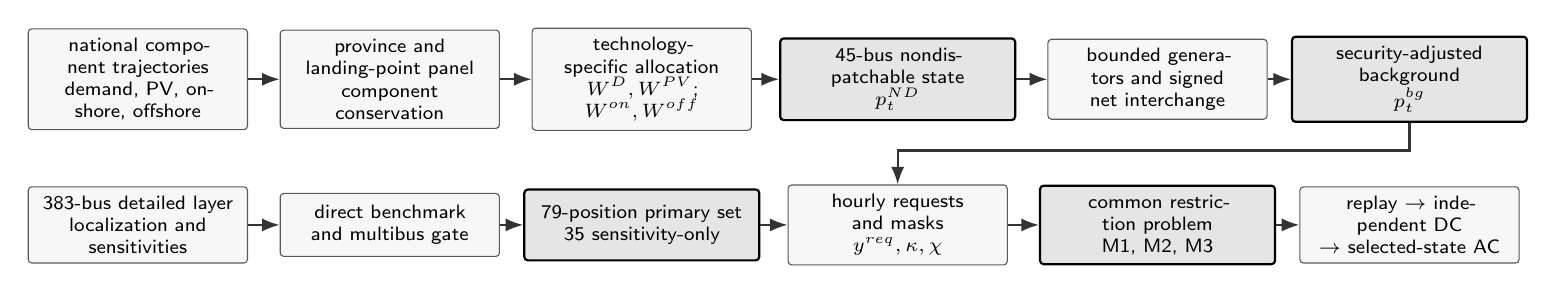
\begin{tikzpicture}[>=Latex,font=\sffamily\scriptsize,
box/.style={draw=black!65,rounded corners=1.3pt,minimum height=.8cm,text width=2.55cm,align=center,fill=black!3},
core/.style={draw=black,rounded corners=1.3pt,minimum height=.9cm,text width=2.75cm,align=center,fill=black!10,line width=.8pt},
arr/.style={->,line width=.75pt,draw=black!80}]
\node[box] (nat) at (0,1.3) {national component trajectories\\demand, PV, onshore, offshore};
\node[box] (prov) at (3.2,1.3) {province and landing-point panel\\component conservation};
\node[box] (alloc) at (6.4,1.3) {technology-specific allocation\\$W^D,W^{PV}$; $W^{on},W^{off}$};
\node[core] (pnd) at (9.65,1.3) {45-bus nondispatchable state\\$p_t^{ND}$};
\node[box] (devices) at (12.95,1.3) {bounded generators and signed net interchange};
\node[core] (pbg) at (16.15,1.3) {security-adjusted background\\$p_t^{bg}$};
\draw[arr] (nat)--(prov); \draw[arr] (prov)--(alloc); \draw[arr] (alloc)--(pnd); \draw[arr] (pnd)--(devices); \draw[arr] (devices)--(pbg);

\node[box] (detailed) at (0,-.55) {383-bus detailed layer\\localization and sensitivities};
\node[box] (gate) at (3.2,-.55) {direct benchmark and multibus gate};
\node[core] (pop) at (6.4,-.55) {79-position primary set\\35 sensitivity-only};
\node[box] (request) at (9.65,-.55) {hourly requests and masks\\$y^{req},\kappa,\chi$};
\node[core] (policy) at (12.95,-.55) {common restriction problem\\M1, M2, M3};
\node[box] (evidence) at (16.15,-.55) {replay $\rightarrow$ independent DC\\$\rightarrow$ selected-state AC};
\draw[arr] (detailed)--(gate); \draw[arr] (gate)--(pop); \draw[arr] (pop)--(request); \draw[arr] (request)--(policy); \draw[arr] (policy)--(evidence);
\draw[arr] (pbg.south) -- ++(0,-.35) -| (request.north);
\end{tikzpicture}}
\caption{Construction and evidence chain. National component totals are disaggregated to provinces or landing points, projected by technology to the 45-bus model, and balanced through bounded public-data devices. The detailed network supplies localization and reduction checks but not policy optimization. Final policies are evaluated through separate replay, DC, and AC layers.}
\label{fig:case_pipeline}
\end{figure*}

\subsection{Contingencies and frozen case}

Candidate line and transformer outages are enumerated from the 45-bus component inventory. A state is retained only when it corresponds to one identifiable modeled element, leaves the EHV network connected, has usable electrical parameters and ratings, and admits a stable affine DC construction. Parallel physical circuits listed separately may be removed one at a time; an aggregated equivalent corridor is not called a single-circuit outage. Islanding states, unsupported devices, missing ratings, and unresolved element semantics are recorded with explicit exclusion reasons.

The final evaluator contains 95 monitored line/transformer elements in the intact state and 93 retained outages. Since the outaged element is absent from its own state, the case contains
\begin{equation}
95+93\times94=8{,}837
\end{equation}
state--element rows per hour. For every state, the artifact stores row and element IDs, orientation, rating source, $\bm H^c$, $\bm h^c$, and $\bm G^c=\bm H^c\bm A$. A 2018 mapped-row reconstruction verifies the intact affine DC network against the independent public reference state where available. This benchmark checks the network construction; it does not make the 2025--2031 scenario paths historical observations.

\begin{table}[t]
\caption{Frozen primary evaluation design}
\label{tab:design}
\centering
\footnotesize
\begin{tabularx}{\columnwidth}{@{}lX@{}}
\toprule
Object & Frozen design \\
\midrule
Chronology & 61,344 hourly intervals, 2025--2031 \\
Operational network & 45 EHV buses; 95 monitored elements \\
Network states & intact plus 93 retained non-islanding outages \\
Row universe & 8,837 state--element rows per hour, checked in both directions \\
Participants & 79 direct primary; 35 multibus sensitivity-only \\
Learning split & 2025--2027 fit; 2028 validation; 2029--2030 held out; 2031 confirmation \\
Allowances & $\rho=0.15$ for M1--M2; $\rho=0.03$ for the M3 mechanism study \\
Rolling controller & 48-h look-ahead; 24-h implementation; no terminal reserve \\
\bottomrule
\end{tabularx}
\end{table}

\subsection{Independent DC and selected-state AC evidence}

Engineering states are selected by a deterministic manifest before independent DC or AC outcomes are viewed. Per evaluation year, the manifest takes the two largest unrestricted-request stress hours, two largest rolling M1--M2 flow-disagreement hours, and two largest annual M2--M3 flow-disagreement hours, followed by deterministic deduplication and fill. For each selected hour it includes the intact state, the worst requested-state outage, and the state with the largest cross-policy flow spread.

The independent DC level sends the exact balanced injection to a separate pandapower/PYPOWER DC execution built from the frozen network element data, taps, phase shifts, and reference-bus convention. A permanent one-to-one map aligns case, state, element, orientation, rating, and row ID. The audit reports MW errors, rating-normalized errors, sign agreement, limiting-element agreement, top-$k$ overlap, and near-limit classification. A false-safe event means the frozen affine evaluator classifies a row as safe while the independent DC execution classifies it as overloaded. This test is an independent software path on the same network data, not an independent dataset.

The selected AC level uses the same manifest and reconstructs the frozen active injection with the validated background reactive state. It reports convergence separately from voltage, thermal, and reactive feasibility. Mapped AC active power is compared with DC active power in MW on the same branch and orientation; AC apparent-power loading is compared only with its AC rating. The audit asks whether nonlinear engineering detail reverses predeclared within-model policy orderings in selected stressed states. It does not establish annual AC-OPF feasibility, full-system N--1 security, or operator validation \cite{Stott2009,Ronellenfitsch2017,Thurner2018}.

\subsection{Experiment hierarchy and baselines}

The numerical design separates theorem evidence from the state-weighting study. At $\rho=0.15$, the required primary cases are annual M1-LP and M2 and rolling M1 and M2 for 2029--2031. M1-LP is not an implementable policy and is never presented as one; it is the strongest continuous lower endpoint implied by the touched-time formulation. Rolling M1 is not treated as an approximation bound produced by a generic heuristic. It is an implementable chronology whose physical rows, materiality decisions, ledger transitions, and final balances are replayed. These two endpoints are more informative than a time-limited annual M1 incumbent because together they locate the unknown annual M1 optimum without assuming that the incumbent is close to it.

At $\rho=0.03$, the required state-weighting cases are annual M2, M3, and M2-MATCHED and rolling M2 and M3. The selected M3 card is compared with three types of ordering control. The PTDF score asks whether a direct one-MW network sensitivity is sufficient. The inverse score tests whether any apparent effect survives reversal of the selected order. The frozen shuffles provide a distribution of arbitrary within-direction orderings under the same amplitude and fitting-reference normalization. These are stronger baselines than a deliberately weak predictor because they isolate three alternative explanations: direct physics, sign-insensitive amplitude, and chance ordering.

The fit and evaluation split enforces nonanticipativity at the card level. Teacher rows and model parameters use 2025--2027. The complete operator problem on 2028 selects the card. Before card serialization, the access audit checks that no 2029--2031 feature, physical input, policy output, rate, or result artifact entered fitting, threshold selection, amplitude selection, or control generation. The frozen card is then evaluated on 2029--2030, with 2031 kept as a separate confirmation. The annual models retain perfect knowledge of their scenario year and are therefore benchmarks rather than online forecasts. The rolling controller uses the same frozen chronology and card but only the current 48-h window and carried balance. Annual and rolling results answer different questions and are not pooled.

Solver performance is also separated from scientific selection. Structural and parameter changes are benchmarked on 2028 before held-out reruns. The accepted implementation may compress active hours, remove provably dominated action coordinates, start from a small directed-row seed, reuse closed row sets and simplex bases, and warm-start overlapping rolling windows. It may not change the physical case, allowance, objective, debit law, numerical acceptance gate, or full-row replay. A faster configuration is accepted only when it reproduces the 2028 M1-LP and M2 values within the frozen tolerances and passes the same debit and physical certificates. This rule prevents runtime tuning from becoming an unreported model change.

Finally, the study reports three reference states before comparing policies. The background index $S_y^{\rm bg}$ measures residual stress in the public-data operating state. The requested-state index $S_y^{\rm req}$ measures the state after prospective transactions but before restriction. The policy index $S_y^M$ measures the post-restriction state. Their separation prevents pre-existing background limitations from being attributed to the accounting rule and shows whether a lower policy value reflects recovery from the prospective request or merely a different baseline.

\section{Numerical Evidence and Interpretation}
\label{sec:results}

The final numerical section is generated from committed V3 artifacts rather than transcribed from solver logs. Every row in Table~\ref{tab:main_results} must share the physical-case hash, participant set, time grid, ratings, and allowance lineage stated above. The policy metrics are: Stage-I residual index $S$; restricted energy $E$ in MWh; physical FDE $\sum_{n,t}\Delta_tx_{n,t}/P_n$; materially touched participant-hours under \eqref{eq:floor}; affected positions and projects; restriction episodes; maximum overload; insecure intervals; solver seconds; and ex-post price-weighted restriction burden
\begin{equation}
B_y^{\rm price}:=
\sum_{n,t}\Delta_t\pi_t x_{n,t},
\label{eq:price_burden}
\end{equation}
where $\pi_t$ is the frozen realized price series. Equation \eqref{eq:price_burden} is a reporting measure, not an optimization objective. Absolute values are reported before percentage changes.

\begin{table*}[t]
\caption{Claim-gated primary outcomes. Dashes are replaced automatically when the final evidence interface is present.}
\label{tab:main_results}
\centering
\footnotesize
\begin{tabular}{@{}llrrrrrr@{}}
\toprule
Period & Policy/certificate & $S$ [MW h row-state] & $E$ [MWh] & Physical FDE [h] & Price burden [EUR] & Touched h & Solver s \\
\midrule
2029--2030 & M2, $\rho=0.15$ & \HeldMTwoS & \HeldMTwoE & -- & -- & -- & -- \\
2029--2030 & annual M1 lower endpoint & \HeldMOneLower & -- & -- & -- & -- & -- \\
2029--2030 & rolling M1 upper endpoint & \HeldMOneUpper & -- & -- & -- & -- & -- \\
2031 & M2, $\rho=0.15$ & \ConfirmMTwoS & -- & -- & -- & -- & -- \\
2031 & annual M1 lower endpoint & \ConfirmMOneLower & -- & -- & -- & -- & -- \\
2031 & rolling M1 upper endpoint & \ConfirmMOneUpper & -- & -- & -- & -- & -- \\
2029--2030 & M3, $\rho=0.03$ & \HeldMThreeS & -- & \HeldMThreeFDE & \HeldMThreeBurden & -- & -- \\
2029--2030 & M2-MATCHED, $\rho=0.03$ & \HeldMMatchedS & -- & \HeldMMatchedFDE & \HeldMMatchedBurden & -- & -- \\
\bottomrule
\end{tabular}
\end{table*}

\subsection{Duration-to-depth comparison}

\ifFinalResultsReady
\emph{Observation.} Across 2029--2030, annual M2 attains $S=\HeldMTwoS$ MW h row-state. The annual M1 optimum lies in the certified interval $[\HeldMOneLower,\HeldMOneUpper]$, and the replay-safe M2 value is separated from the M1-LP lower endpoint by \HeldCertMargin\ MW h row-state after numerical margins. In 2031, the corresponding M2 value is \ConfirmMTwoS\ and the M1 interval is $[\ConfirmMOneLower,\ConfirmMOneUpper]$. These are absolute objective values; any percentage reduction is reported only beside them.

\emph{Mechanism.} The source-of-separation identity \eqref{eq:debit_gap} is evaluated on the fixed M2 and M1-LP trajectories and binned by request headroom $\bar x/P$. A concentration of the debit gap in low-request coordinates indicates that touched-time accounting charges a large fraction of one token for physically shallow actions. Near-full-request coordinates contribute little because $\bar x\approx P$. Directional and seasonal decompositions are descriptive accounting identities, not causal attributions.

\emph{Implication.} When \eqref{eq:strict_certificate} passes, the conclusion is stronger than a comparison with a rolling policy or a time-limited annual M1 incumbent: no feasible annual M1 schedule can attain the M2 Stage-I value. When the certificate does not pass, the paper reports only the interval and does not infer equality or superiority.
\else
The duration-to-depth prose is complete, but numerical statements are intentionally suppressed in this pre-results build. The final campaign must populate the absolute M2 value, the M1-LP lower endpoint, the rolling-M1 upper endpoint, and the strict numerical margin before this subsection is released for submission.
\fi

\begin{figure}[t]
\centering
\IfFileExists{figures/fig_m1_certificate.pdf}{%
\includegraphics[width=\columnwidth]{figures/fig_m1_certificate.pdf}}{%
\fbox{\parbox[c][3.1cm][c]{0.92\columnwidth}{\centering
Final artifact: annual M2 exact value and annual M1 interval for 2029, 2030, and 2031.\\[1mm]
No cumulative curve is labeled a pointwise bound.}}}
\caption{Annual duration-to-depth certificate. The final figure reports absolute Stage-I values and the scalar M1 interval by year.}
\label{fig:m1_certificate}
\end{figure}

The rolling comparison answers a separate question: how much of the annual advantage transfers to an unpaced 48/24-h controller with no terminal entitlement value. The held-out rolling totals are \HeldRollingMOneS\ for M1 and \HeldRollingMTwoS\ for M2 when the result interface is present. A smaller rolling difference than the annual certificate is interpreted as an online allocation effect, not a contradiction of the feasible-set theorem. The theorem compares annual optima; the rolling controller acts with a truncated horizon and carries only the remaining balance.

\subsection{State-conditioned debit and matched exposure}

\ifFinalResultsReady
\emph{Observation.} At $\rho=0.03$, the held-out Stage-I values are \HeldMTwoRhoThreeS\ for M2, \HeldMThreeS\ for the selected M3 card, and \HeldMMatchedS\ for M2-MATCHED. M3 realizes \HeldMThreeFDE\ participant-hours of physical FDE, while the matched comparator receives the same participant-specific vector by construction. The ex-post price burdens are EUR~\HeldMThreeBurden\ and EUR~\HeldMMatchedBurden, respectively.

\emph{Mechanism.} The difference between M2 and M3 is decomposed according to \eqref{eq:matched_decomposition}. The exposure term measures the consequence of changing each participant's effective physical allowance. The nonnegative shape penalty measures the restriction imposed by the frozen state-dependent weighting relative to uniform depth at the same participant-specific exposure. The selected card is described as improving state allocation only if a positive gain remains after the matched comparison and survives the predeclared PTDF, inverse, and 32-shuffle controls.

\emph{Implication.} A lower nominal M3 value accompanied by greater physical FDE but no matched-exposure gain supports a narrow conclusion: debit weighting changes effective entitlement but does not improve allocation once exposure is held fixed. Conversely, a positive matched-exposure gain that also exceeds the control distribution supports a state-ordering claim. The paper retains either outcome.
\else
The final M3 conclusion is claim-gated. It requires the corrected Stage-II teacher, the frozen F0 card, M2-MATCHED, the complete control family, and the absolute physical-FDE and price-burden values. No statement about the value of state weighting is made in this pre-results build.
\fi

\begin{figure*}[t]
\centering
\IfFileExists{figures/fig_m3_and_engineering.pdf}{%
\includegraphics[width=0.94\textwidth]{figures/fig_m3_and_engineering.pdf}}{%
\fbox{\parbox[c][3.55cm][c]{0.94\textwidth}{\centering
Left panel: M2--M3--M2-MATCHED exposure/shape decomposition with PTDF, inverse, and 32-shuffle controls.\qquad
Right panel: mapped DC--AC active-power agreement and selected-state feasibility counts.\\[1mm]
All axes use absolute engineering units; AC MVA is not placed on a one-to-one line against DC MW.}}}
\caption{State-conditioned mechanism and engineering evidence. The final figure combines the matched-exposure diagnosis with the predeclared selected-state DC/AC audit.}
\label{fig:m3_engineering}
\end{figure*}

Rate-bound results are reported for $[0.7,1.3]$, $[0.5,1.5]$, and $[0.25,2.0]$. The three-point amplitude check $\gamma\in\{0.7,1.0,1.3\}$ is run before the full path. The full path is included only if all exact cases complete and the endpoints reproduce flat M2 and the frozen selected card. Fixed-policy seven-day block resampling, when shown, describes temporal concentration conditional on already optimized trajectories. It is not an optimization-gap interval or a participant-resampling argument.

\subsection{Physical and computational checks}

The independent DC gate is numerical rather than statistical because both paths encode the same DC equations. The final report supplies the maximum mapped-row error \IndependentDCMaxError\ MW and \IndependentDCFalseSafe\ false-safe cases. Any mapping failure or false-safe classification above tolerance blocks row-level physical claims. The selected AC audit then reports a convergence share of \SelectedACConvergence\ and \SelectedACReversals\ policy-order reversals when the result interface is present. Convergence, voltage feasibility, thermal feasibility, and reactive feasibility remain separate counts.

The final solver table reports model construction time, active hours, candidate and retained action coordinates, initial and closed row counts, nonzeros, closure rounds, Stage-I and Stage-II seconds, peak memory, and replay seconds. Annual cases are expected to fall in the measured range \AnnualRuntimeRange\ s and rolling policy-years in \RollingRuntimeRange\ s after the 2028 performance regression is frozen. Speed changes are accepted only when the optimized implementation reproduces the same $S$, $E$, debit, row closure, and replay within the declared tolerances. Presolve and thread choices are treated as solver settings, not mathematical assumptions; they are benchmarked against memory and certificate behavior rather than selected for appearance.

\section{Scope and Limitations}
\label{sec:limitations}

The theorem concerns accounting geometry under a common physical set. It does not show that M2 and M1 protect the same legal service, that one service should receive the same tariff, or that the Stage-I objective captures all customer and system costs. Price-weighted burden in \eqref{eq:price_burden} is ex post and does not turn the policy into a welfare optimization.

The annual models use the complete frozen hourly chronology but perfect knowledge of the scenario path. The rolling experiment removes that annual foresight only through a deterministic 48/24-h controller; it is not a stochastic program and provides no probabilistic guarantee. Scenario demand, renewable production, and requests are not authenticated forecast vintages. No storage, commitment, ramping, or minimum up/down constraints are present. These omissions matter if operational flexibility is materially constrained across hours beyond the entitlement ledger.

The 45-bus public-data model is not an operator digital twin. The primary population excludes 35 multibus positions because the all-or-none reduction gate does not admit the full set. The outage claim covers retained supported non-islanding elements only. The DC parent ignores voltage and reactive power; selected-state AC tests bound the interpretation but do not prove annual AC feasibility. The security-adjusted background is reproducible but is not observed TSO dispatch. M3 uses a narrow F0 feature family because richer residual-load features lack archived D--1 provenance. A flat or weak M3 result is therefore informative about this specified card construction, not every possible state-dependent product.

\section{Conclusion}
\label{sec:conclusion}

Partial restriction turns annual entitlement accounting into an operational design choice. Touched time limits the support of intervention and becomes depth-blind after an interval is opened. Proportional depth limits cumulative normalized physical exposure. The exact M1-LP projection makes this distinction formal: under the same physical model and allowance, the projected touched-time relaxation is contained in M2. A replay-feasible M2 value below the M1-LP lower bound therefore certifies a strictly lower Stage-I residual index than every feasible annual M1 schedule, while a complete rolling-M1 trajectory supplies the opposite endpoint of the annual bracket.

State-dependent weighting requires a different standard. The M3 card is frozen from an exact Stage-II M2 teacher and provenance-safe information, then evaluated with M2-MATCHED and predeclared controls. This prevents a larger effective physical entitlement from being mislabeled as better state allocation. The Dutch case preserves spatial demand and renewable components through province-to-bus projection and separates the DC parent model from independent DC and selected-state AC evidence.

\ifFinalResultsReady
The final numerical conclusion is inserted from the claim-gated artifacts: the held-out M2 value is \HeldMTwoS\ MW h row-state, the annual M1 interval is $[\HeldMOneLower,\HeldMOneUpper]$, and the M3 matched-exposure outcome is reported without changing its sign or scale.
\else
The theoretical, physical, and evidence contracts are complete. Final numerical sentences remain withheld until the frozen campaign, replay, and engineering gates close.
\fi

\bibliographystyle{IEEEtran}
\bibliography{references}
\end{document}
